%&latex
\documentclass[12pt]{article}
\usepackage{amsmath}
\usepackage{graphicx,psfrag,epsf}
\usepackage{enumerate}
\usepackage{natbib}
\usepackage{url} % not crucial - just used below for the URL

% Additional packages
\usepackage{algorithm2e}
\usepackage{float}
\usepackage{hyperref}

% Setup hyperlinks
\hypersetup{
  colorlinks=true,
  linkcolor=blue,
  citecolor=blue,      
  urlcolor=blue 
}

%\pdfminorversion=4
% NOTE: To produce blinded version, replace "0" with "1" below.
\newcommand{\blind}{0}

%
\newcommand{\pkg}[1]{\texorpdfstring%
{{\normalfont\fontseries{b}\selectfont #1}}%
{#1}}
\newcommand{\file}[1]{{`\normalfont\textsf{#1}'}}

\def\code#1{\texttt{#1}}
\def\pkg#1{\textbf{\texttt{#1}}}
\def\ref#1{\textbf{(#1)}}

\DeclareMathOperator{\flatness}{flatness}
\DeclareMathOperator{\imp}{imp}
\DeclareMathOperator{\inter}{int}

% DON'T change margins - should be 1 inch all around.
\addtolength{\oddsidemargin}{-.5in}%
\addtolength{\evensidemargin}{-.5in}%
\addtolength{\textwidth}{1in}%
\addtolength{\textheight}{1.3in}%
\addtolength{\topmargin}{-.8in}%


\begin{document}

%\bibliographystyle{natbib}

\def\spacingset#1{\renewcommand{\baselinestretch}%
{#1}\small\normalsize} \spacingset{1}


%%%%%%%%%%%%%%%%%%%%%%%%%%%%%%%%%%%%%%%%%%%%%%%%%%%%%%%%%%%%%%%%%%%%%%%%%%%%%%

\if0\blind
{
  \title{\bf A Simple and Effective Model-Based Variable Importance Measure}
  \author{Brandon M. Greenwell\thanks{
    The authors gratefully acknowledge \textit{please remember to list all relevant funding sources in the unblinded version}}\hspace{.2cm}\\
    Illumination Works           \\
    and \\
    Andrew J. McCarthy \\
    The Perduco Group \\
    and \\
    Bradley C. Boehmke \\
    Department of Operational Sciences, Air Force Institute of Technology}
  \maketitle
} \fi

\if1\blind
{
  \bigskip
  \bigskip
  \bigskip
  \begin{center}
    {\LARGE\bf Title}
\end{center}
  \medskip
} \fi

\bigskip
\begin{abstract}
In the era of "big data", it is becoming more of a challenge to not only build state-of-the-art predictive models, but also gain an understanding of what's really going on in the data. For example, it is often of interest to know which, if any, of the predictors in a fitted model are relatively influential on the predicted outcome. Some modern algorithms---like random forests and boosted decision trees---have a natural way of quantifying the importance or relative influence of each feature. Other algorithms---like naive Bayes classifiers and support vector machines---are not capable of doing so and model-free approaches are generally used to measure each predictor's importance. In this paper, we discuss a model-based approach to measuring predictor importance in any supervised learning setting. The R code to reproduce all of the figures in this paper is available in the supplementary materials.
\end{abstract}

\noindent%
{\it Keywords:} Relative influence, Interaction effect, Partial dependence function, Partial dependence plot, PDP.
\vfill

\newpage
\spacingset{1.45} % DON'T change the spacing!


%%%%%%%%%%%%%%%%%%%%%%%%%%%%%%%%%%%%%%%%%%%%%%%%%%%%%%%%%%%%%%%%%%%%%%%%%%%%%%%%
\section{Introduction}
\label{sec:introduction}
%%%%%%%%%%%%%%%%%%%%%%%%%%%%%%%%%%%%%%%%%%%%%%%%%%%%%%%%%%%%%%%%%%%%%%%%%%%%%%%%

Complex supervised learning algorithms, such as neural networks and support vector machines, are more common than ever in predictive analytics, especially when dealing with large observational databases that don't adhere to the strict assumptions imposed by traditional statistical techniques (e.g., multiple linear regression which typically assumes linearity, homoscedasticity, and normality). However, it can be challenging to understand the results of such complex models and explain them to management. Graphical displays such as variable importance plots (when available) and partial dependence plots (PDPs) offer a simple solution. 

PDPs are low-dimensional graphical renderings of the prediction function $\widehat{f}\left(\boldsymbol{x}\right)$ so that the relationship between the outcome and predictors of interest can be more easily understood. These plots are especially useful in explaining the output from "black box" models. While PDPs can be constructed for any predictor in a fitted model, variable importance scores are more difficult to define. What does it mean for a feature to be important? It's influence on the predicted outcome? Some methods---like random forests and other tree-based methods---have a natural way of defining variable importance. In this paper, we consider a partial dependence-based variable importance measure that can be used with any supervised learning algorithm. Furthermore, we show how this new method can also be used to quantify the strength of potential interaction effects.


%%%%%%%%%%%%%%%%%%%%%%%%%%%%%%%%%%%%%%%%%%%%%%%%%%%%%%%%%%%%%%%%%%%%%%%%%%%%%%%%
\section{Background}
\label{sec:background}
%%%%%%%%%%%%%%%%%%%%%%%%%%%%%%%%%%%%%%%%%%%%%%%%%%%%%%%%%%%%%%%%%%%%%%%%%%%%%%%%

We are often confronted with the task of extracting knowledge from large databases. For this task we turn to various statistical learning algorithms which, when tuned correctly, can have state-of-the-art predictive performance. However, having a model that predicts well is only solving part of the problem. It is also desirable to extract information about the relationships uncovered by the learning algorithm. For instance, we often want to know which predictors, if any, are important by assigning some type of variable importance score to each feature. Once a set of influential features has been identified, the next step is summarizing the functional relationship between each feature, or subset thereof, and the outcome of interest. However, since most statistical learning algorithms are "black box" models, extracting this information is not always straightforward. Luckily, some learning algorithms have a natural way of defining variable importance.


%%%%%%%%%%%%%%%%%%%%%%%%%%%%%%%%%%%%%%%%%%%%%%%%%%%%%%%%%%%%%%%%%%%%%%%%%%%%%%%%
\subsection{Model-based approaches to variable importance}
\label{sec:model-based-vi}
%%%%%%%%%%%%%%%%%%%%%%%%%%%%%%%%%%%%%%%%%%%%%%%%%%%%%%%%%%%%%%%%%%%%%%%%%%%%%%%%

Decision trees probably offer the most natural model-based approach to quantifying the importance of each feature. In a binary decision tree, at each node $t$, a single predictor is used to partition the data into two homogeneous groups. The chosen predictor is the one that maximizes some measure of improvement $\widehat{i}_t$. The relative importance of predictor $x$ is the sum of the squared improvements over all internal nodes of the tree for which $x$ was chosen as the partitioning variable; see \citet{classification-breiman-1984} for details. This idea also extends to ensembles of decision trees, such as boosting and random forest. In ensembles, the improvement score for each predictor is averaged across all the trees in the ensemble. Fortunately, due to the stabilizing effect of averaging, the improvement-based variable importance metric is often more reliable in large ensembles \citep[pg. 368]{hastie-elements-2009}. Random forests offer an additional method for computing variable importance scores. The idea is to use the leftover out-of-bag (OOB) data to construct validation-set errors for each tree. Then, each predictor is randomly shuffled in the OOB data and the error is computed again. The idea is that if variable $x$ is important, then the validation error will go up when $x$ is perturbed in the OOB data. The difference in the two errors is recorded for the OOB data then averaged across all trees in the forest.

In multiple linear regression, the absolute value of the $t$-statistic is commonly used as a measure of variable importance. The same idea also extends to generalized linear models and nonlinear least squares. Multivariate adaptive regression splines (MARS), which were introduced in \citet{friedman-1991-mars}, is an automatic and adaptive regression technique which can be seen as a generalization of multiple linear regression and generalized linear models. In the MARS algorithm, the contribution (or variable importance score) for each predictor is determined using a generalized cross-validation (GCV) statistic.

For neural networks, two popular methods for constructing variable importance scores are the Garson algorithm \citep{interpreting-garson-1991}, later modified by \citet{back-goh-1995}, and the Olden algorithm \citep{accurate-olden-2004}. For both algorithms, the basis of these importance scores is the network's connection weights. The Garson algorithm determines variable importance by identifying all weighted connections between the nodes of interest. Olden's algorithm, on the other hand, uses the product of the raw connection weights between each input and output neuron and sums the product across all hidden neurons. This has been shown to outperform the Garson method in various simulations.


%%%%%%%%%%%%%%%%%%%%%%%%%%%%%%%%%%%%%%%%%%%%%%%%%%%%%%%%%%%%%%%%%%%%%%%%%%%%%%%%
\subsection{Filter-based approaches to variable importance}
%%%%%%%%%%%%%%%%%%%%%%%%%%%%%%%%%%%%%%%%%%%%%%%%%%%%%%%%%%%%%%%%%%%%%%%%%%%%%%%%

Filter-based approaches, which are described in \citet[chap. 18]{applied-kuhn-2013}, do not make use of the fitted model to measure variable importance. They also do not take into account the other predictors in the model.

For regression problems, a popular approach to measuring the variable importance of a numeric predictor $x$ is to first fit a flexible nonparametric model between $x$ and the target $Y$; for example, the locally-weighted polynomial regression (LOWESS) method developed by \citet{robust-cleveland-1979}. From this fit, a pseudo-$R^2$ measure can be obtained from the resulting residuals and used as a measure of variable importance. For categorical predictors, a different method based on standard statistical tests (e.g., $t$-tests and ANOVAs) is employed; see \citet[chap. 18]{applied-kuhn-2013} for details.

For classification problems, an area under the ROC curve (AUC) statistic can be used to quantify predictor importance. The AUC statistic is computed by using the predictor $x$ as input to the ROC curve. If $x$ can reasonably separate the classes of $Y$, then that is a clear indicator that $x$ is an important predictor (in terms of class separation) and this is captured in the corresponding AUC statistic. For problems with more than two classes, extensions of the ROC curve or a one-vs-all approach can be used.


%%%%%%%%%%%%%%%%%%%%%%%%%%%%%%%%%%%%%%%%%%%%%%%%%%%%%%%%%%%%%%%%%%%%%%%%%%%%%%%%
\subsection{Partial dependence plots}
%%%%%%%%%%%%%%%%%%%%%%%%%%%%%%%%%%%%%%%%%%%%%%%%%%%%%%%%%%%%%%%%%%%%%%%%%%%%%%%%

\citet{harrison-1978-hedonic} analyzed a dataset containing suburban Boston housing data from the 1970 census. They sought a housing value equation using an assortment of features; see \citet[Table IV]{harrison-1978-hedonic} for a description of each variable. The usual regression assumptions, such as normality, linearity, and constant variance, were clearly violated, but through an exhausting series of transformations, significance testing, and grid searches, they were able to build a model which fit the data reasonably well ($R^2 = 0.81$). Their prediction equation is given in Equation~\eqref{eqn:boston}. This equation makes interpreting the model easier. For example, the average number of rooms per dwelling ($RM$) is included in the model as a quadratic term with a positive coefficient. This means that there is a monotonic increasing relationship between $RM$ and the predicted median home value, but larger values of $RM$ have a greater impact.
\begin{equation}
\label{eqn:boston}
\begin{aligned}
\widehat{\log\left(MV\right)} &= 9.76 + 0.0063 RM^2 + 8.98\times10^{-5} AGE - 0.19\log\left(DIS\right) + 0.096\log\left(RAD\right) \\
  & \quad - 4.20\times10^{-4} TAX - 0.031 PTRATIO + 0.36\left(B - 0.63\right)^2 - 0.37\log\left(LSTAT\right) \\
  & \quad - 0.012 CRIM + 8.03\times10^{-5} ZN + 2.41\times10^{-4} INDUS + 0.088 CHAS \\
  & \quad - 0.0064 NOX^2.
\end{aligned}
\end{equation}

However, classical regression and model building is rather ill-suited for more contemporary datasets, like the Ames housing data described in \citet{ames-cock-2011} which has a total of 79 predictors (and many more that can be created through feature engineering). Fortunately, using modern computing power, many supervised learning algorithms can fit such datasets in seconds, producing powerful, highly accurate models. The downfall of many of these machine learning algorithms, however, is decreased interpretability. Unlike prediction formulas such as Equation~\eqref{eqn:boston}, many machine learning algorithms are left attempting to convey some relative measure of variable importance which provide insight, but cannot match the simplicity of Equation~\eqref{eqn:boston} and others like it.

Quantifying the importance of each predictor is a crucial task in any supervised learning problem, but to gain even more insight, we can construct partial dependence plots (PDPs); see \citet{friedman-2001-greedy} for details. PDPs are particularly effective at helping to explain the output from "black box" models, such as random forests and support vector machines. Not only do PDPs visually convey the relationship between low cardinality subsets of the feature set (usually 1-3) and the response (while accounting for the average effect of the other predictors in the model), they can also be used to rank and score the predictors in terms of their relative influence on the predicted outcome, as will be demonstrated in this paper. 

Let $\boldsymbol{x} = \left\{x_1, x_2, \dots, x_p\right\}$ represent the predictors in a model whose prediction function is $\widehat{f}\left(\boldsymbol{x}\right)$. If we partition $\boldsymbol{x}$ into an interest set, $\boldsymbol{z}_s$, and its complement, $\boldsymbol{z}_c = \boldsymbol{x} \setminus \boldsymbol{z}_s$, then the "partial dependence" of the response on $\boldsymbol{z}_s$ is defined as
\begin{equation}
\label{eqn:avg_fun}
  f_s\left(\boldsymbol{z}_s\right) = E_{\boldsymbol{z}_c}\left[\widehat{f}\left(\boldsymbol{z}_s, \boldsymbol{z}_c\right)\right] = \int \widehat{f}\left(\boldsymbol{z}_s, \boldsymbol{z}_c\right)p_{c}\left(\boldsymbol{z}_c\right)d\boldsymbol{z}_c,
\end{equation}
where $p_{c}\left(\boldsymbol{z}_c\right)$ is the marginal probability density of $\boldsymbol{z}_c$: $p_{c}\left(\boldsymbol{z}_c\right) = \int p\left(\boldsymbol{x}\right)d\boldsymbol{z}_s$.
Equation~\eqref{eqn:avg_fun} can be estimated from a set of training data by
\begin{equation}
\label{eqn:pdf}
\bar{f}_s\left(\boldsymbol{z}_s\right) = \frac{1}{n}\sum_{i = 1}^n\widehat{f}\left(\boldsymbol{z}_s,\boldsymbol{z}_{i, c}\right),
\end{equation}
where $\boldsymbol{z}_{i, c}$ $\left(i = 1, 2, \dots, n\right)$ are the values of $\boldsymbol{z}_c$ that occur in the training sample; that is, we average out the effects of all the other predictors in the model.

Constructing a PDP \eqref{eqn:pdf} in practice is rather straightforward. To simplify, let $\boldsymbol{z}_s = x_1$ be the predictor variable of interest with unique values $\left\{x_{11}, x_{12}, \dots, x_{1k}\right\}$. The partial dependence of the response on $x_1$ can be constructed as follows:
\begin{algorithm}
  \textbf{Input}: the unique predictor values $x_{11}, x_{12}, \dots, x_{1k}$;

  \textbf{Output}: the estimated partial dependence values $\bar{f}_1\left(x_{11}\right), \bar{f}_1\left(x_{12}\right), \dots, \bar{f}_1\left(x_{1k}\right)$. \BlankLine
  \For{$i \in \left\{1, 2, \dots, k\right\}$}{
    \BlankLine
    (1) copy the training data and replace the original values of $x_1$ with the constant $x_{1i}$;
    \BlankLine
    (2) compute the vector of predicted values from the modified copy of the training data;
    \BlankLine
    (3) compute the average prediction to obtain $\bar{f}_1\left(x_{1i}\right)$.\BlankLine}
    \BlankLine
    % Plot the pairs $\left\{x_{1i}, \bar{f}_1\left(x_{1i}\right)\right\}$ for $i = 1, 2, \dotsc, k$.
    \BlankLine
  \caption{A simple algorithm for constructing the partial dependence of the response on a single predictor $x_1$. \label{alg:pdp}}
\end{algorithm}
% \newline

The PDP for $x_1$ is obtained by plotting the pairs $\left\{x_{1i}, \bar{f}_1\left(x_{1i}\right)\right\}$ for $i = 1, 2, \dotsc, k$. Algorithm~\ref{alg:pdp} can be computationally expensive since it involves $k$ passes over the training records. Some ideas are discussed in \citet{pdp-greenwell-2017}. Most importantly, Algorithm~\ref{alg:pdp} is embarrassingly parallel and computing partial dependence functions for each predictor can be done rather quickly on a machine with a multi-core processor. For much larger datasets, it may be worthwhile to reduce the grid size by using specific quantiles for each predictor, rather than using all the unique observations. For example, the partial dependence function can be approximated very quickly by using the min and max of each predictor along with the deciles of the unique predictor values. The exception is classification and regression trees based on single-variable splits which can make use of the efficient weighted tree traversal method described in \citet{friedman-2001-greedy}.

While PDPs are an invaluable tool in understanding the relationships uncovered by complex nonparametric models, they can be misleading in the presence of substantial interaction effects \citep{goldstein-peeking-2015}. To overcome this issue, \citeauthor{goldstein-peeking-2015} developed the concept of individual conditional expectation (ICE) curves. ICE curves display the estimated relationship between the response and a predictor of interest for each observation; in other words, skipping step 1 (c) in Algorithm~\ref{alg:pdp}. Consequently, the PDP for a predictor of interest can be obtained by averaging the corresponding ICE curves across all observations. Although ICE curves provide a refinement over traditional PDPs in the presence of substantial interaction effects, in Section~\ref{sec:interaction}, we show how to use partial dependence functions to evaluate the strength of potential interactions effects.


%%%%%%%%%%%%%%%%%%%%%%%%%%%%%%%%%%%%%%%%%%%%%%%%%%%%%%%%%%%%%%%%%%%%%%%%%%%%%%%%
\subsection{The Ames housing dataset}
\label{sec:ames}
%%%%%%%%%%%%%%%%%%%%%%%%%%%%%%%%%%%%%%%%%%%%%%%%%%%%%%%%%%%%%%%%%%%%%%%%%%%%%%%%

For illustration, we will use the Ames housing dataset described in \citep{ames-cock-2011}---a modernized and expanded version of the often cited Boston Housing dataset \citep{harrison-1978-hedonic}. These data are available from Kaggle: \url{https://www.kaggle.com/c/house-prices-advanced-regression-techniques/data}. Using the R package \pkg{h2o} \citep{h2o-pkg}, we trained and tuned a gradient boosted model (GBM) \citep{friedman-2001-greedy} using 10-fold cross-validation. The model fit is reasonable, with a cross-validated (pseudo) $R^2$ of 90.06\%. Like other tree-based ensembles, GBMs have a natural way of defining variable importance which was described in Section~\ref{sec:model-based-vi}. The top 15 GBM-based variable importance scores are displayed in Figure~\ref{fig:ames-gbm-vip}. This plot indicates that the overall quality of the material and finish of the house (\code{OverallQual}), physical location within the Ames city limits (\code{Neighborhood}), and the above grade (ground) living area (\code{GrLivArea}) are highly associated with the logarithm of the sales price (\code{LogSalePrice}). The variable importance scores also indicated that the slope of the property (\code{LandSlope}), the dollar value of miscellaneous features (\code{MiscVal}), and the presence of miscellaneous features (\code{MiscFeature})  have little association with \code{LogSalePrice}.
\begin{figure}[!htb]
  \centering
  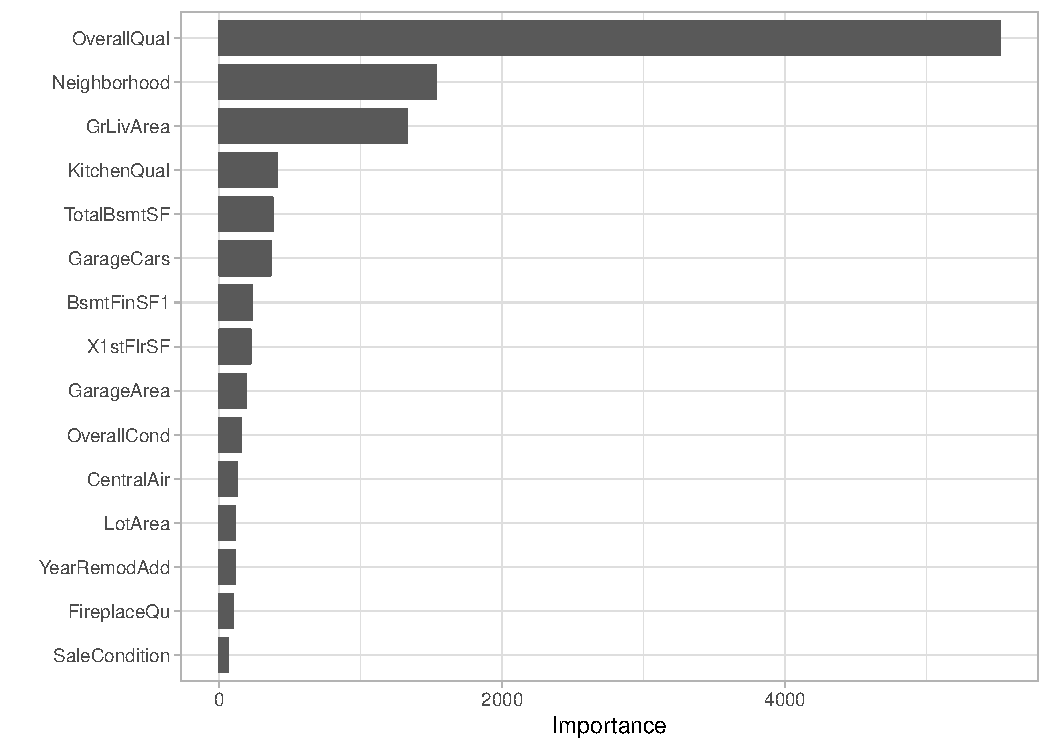
\includegraphics[width=1.0\textwidth]{ames-gbm-vip}
  \caption{Variable importance scores from a random forest fit to the (corrected) Boston housing data. \textit{Left}: OOB-based variable importance scores. \textit{Right}: Impurity-based variable importance scores. \label{fig:ames-gbm-vip}}
\end{figure}

The PDPs for these six variables are displayed in Figure~\ref{fig:ames-gbm-pdps}. These plots indicate that \code{OverallQual}, \code{Neighborhood}, and \code{GrLivArea} have a strong nonlinear relationship with the predicted outcome. For instance, it seems that above grade living area has a monotonically increasing relationship with sale price until about 12 square feet, after which the relationship flattens out. Notice how the PDPs for \code{LandSlope}, \code{MiscVal}, and \code{MiscFeature} are relatively flat in comparison. It is this notion of ``flatness'' which we will use as a basis to define our variable importance measure.
\begin{figure}[H]
  \centering
  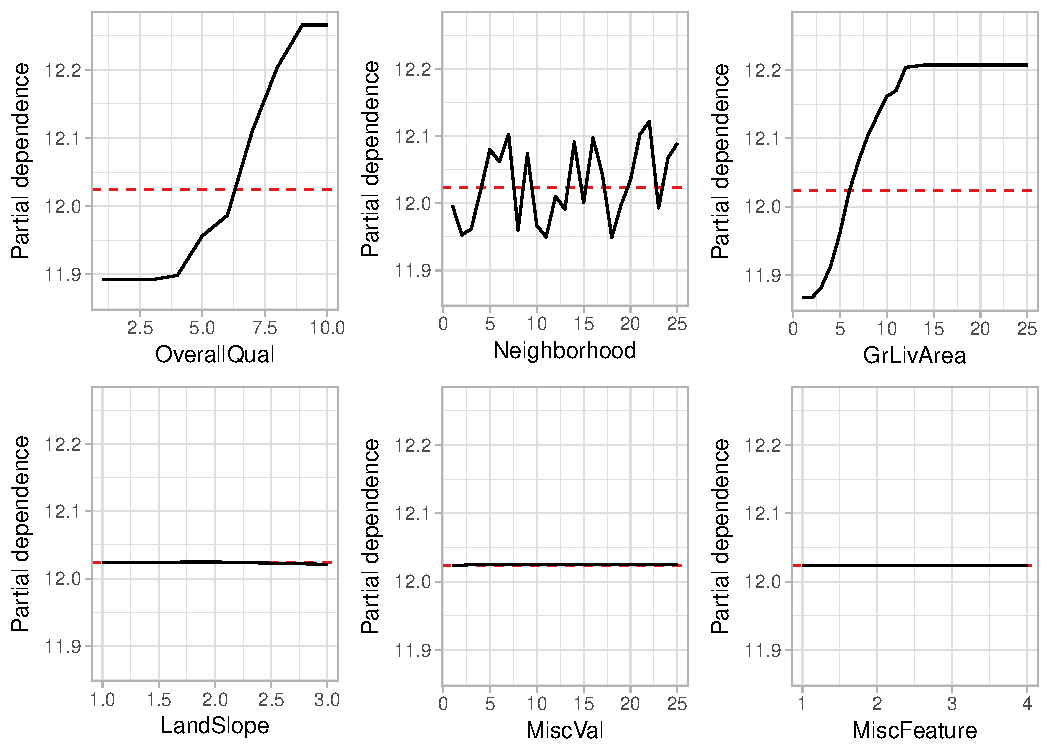
\includegraphics[width=1.0\textwidth]{ames-gbm-pdps}
  \caption{Partial dependence of \code{cmedv} on \code{lstat} (left), \code{rm} (middle), and \code{zn} (right). The mean of the $n = 506$ median home values is indicated by a dashed red line. \label{fig:ames-gbm-pdps}}
\end{figure}


%%%%%%%%%%%%%%%%%%%%%%%%%%%%%%%%%%%%%%%%%%%%%%%%%%%%%%%%%%%%%%%%%%%%%%%%%%%%%%%%
\section{A partial dependence-based variable importance measure}
\label{sec:new}
%%%%%%%%%%%%%%%%%%%%%%%%%%%%%%%%%%%%%%%%%%%%%%%%%%%%%%%%%%%%%%%%%%%%%%%%%%%%%%%%

The PDP for \code{zn} in Figure~\ref{fig:ames-gbm-pdps} is relatively flat (i.e., near-zero slope), indicating that \code{zn} does not have much influence on the predicted median home value. In other words, the partial dependence values $\bar{f}_i\left(x_{ij}\right)$ $\left(j = 1, 2, \dots, k_i\right)$ display little variability. One might conclude that any variable for which the PDP is "flat" is likely to be less important than those predictors whose PDP varies across a wider range of the response.

Our notion of variable importance is based on any measure of the "flatness" of the partial dependence function. In general, we define
\begin{equation*}
  \imp\left(x\right) = \flatness\left(\bar{f}_s\left(\boldsymbol{z}_s\right)\right),
\end{equation*}
where $\flatness$ is any measure of "flatness" of the curve. A simple and effective measure to use is the sample standard deviation for continuous predictors and the range statistic (divided by 4) for factors with $K$ levels. Based on Algorithm~\ref{alg:pdp}, our importance measure for predictor $x_1$ is simply
\begin{equation}
\label{eqn:vi}
  \imp\left(x_1\right) = 
  \begin{cases}
    \sqrt{\frac{1}{k - 1}\sum_{i = 1}^k\left[\bar{f}_1\left(x_{1i}\right) - \frac{1}{k}\sum_{i = 1}^k\bar{f}_1\left(x_{1i}\right)\right] ^ 2} & \quad \text{if } x_1 \text{ is continuous}\\
    \left[\max_i\left(\bar{f}_1\left(x_{1i}\right)\right) - \min_i\left(\bar{f}_1\left(x_{1i}\right)\right)\right] / 4 & \quad \text{if } x_1 \text{ is categorical}
  \end{cases}.
\end{equation}
Note that our variable importance metric relies on the fitted model; hence, it is crucial to properly tune and train the model to have good performance.

To illustrate, we applied Algorithm~\ref{alg:pdp} to all of the predictors in the GBM for the Ames housing example and computed \eqref{eqn:vi}. The results are displayed in Figure~\ref{fig:ames-gbm-vip-pd}. In this case, our partial dependence-based algorithm matches closely with the results from the random forest. In particular, Figure~\ref{fig:ames-gbm-vip-pd} shows that \code{rm} and \code{lstat} are, by far, the most important variables in predicting median home value, while the predictors \code{zn}, \code{rad}, \code{lat}, and \code{b} seem to be the least important.

\begin{figure}[!htb]
  \centering
  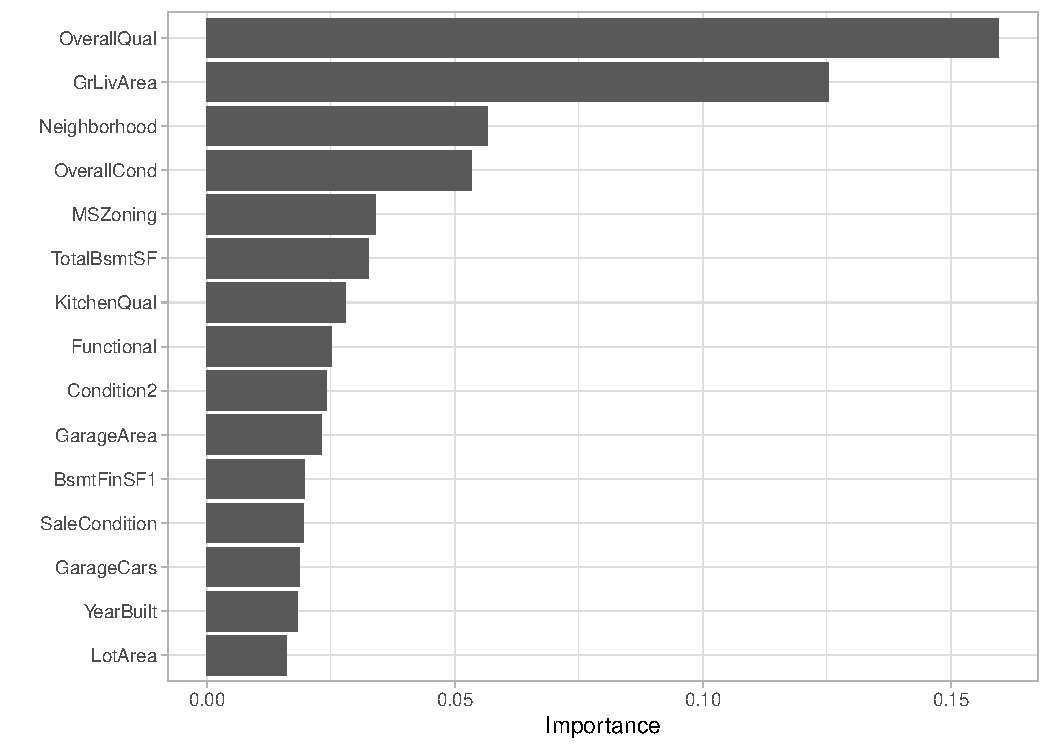
\includegraphics[width=1.0\textwidth]{ames-gbm-vip-pd}
  \caption{Partial-dependence-based variable importance scores from a GBM fit to the Ames housing data. \label{fig:ames-gbm-vip-pd}}
\end{figure}


%%%%%%%%%%%%%%%%%%%%%%%%%%%%%%%%%%%%%%%%%%%%%%%%%%%%%%%%%%%%%%%%%%%%%%%%%%%%%%%%
\subsection{Linear models}
\label{sec:linear}
%%%%%%%%%%%%%%%%%%%%%%%%%%%%%%%%%%%%%%%%%%%%%%%%%%%%%%%%%%%%%%%%%%%%%%%%%%%%%%%%

As mentioned earlier, a natural choice for measuring the importance of each term in a linear model is to use the absolute value of the corresponding coefficient divided by its estimated standard error (i.e., the absolute value of the $t$-statistic). This turns out to be equivalent to the partial dependence-based metric \eqref{eqn:vi} when the predictors are independently and uniformly distributed over the same range.

For example, suppose we have a linear model of the form
\begin{equation*}
  Y = \beta_0 + \beta_1 X_1 + \beta_2 X_2 + \epsilon,
\end{equation*}
where $\beta_i$ ($i = 1, 2$) is a constant, $X_1$ and $X_2$ are both $\mathcal{U}\left(0, 1\right)$ random variables, and $\epsilon \sim \mathcal{N}\left(0, \sigma ^ 2\right)$. Since we know the distribution of $X_1$ and $X_2$, we can easily find $f_1\left(X_1\right)$ and $f_2\left(X_2\right)$. For instance, 
\begin{equation*}
  f_1\left(X_1\right) = \int_0^1 E\left[Y | X_1, X_2\right] p\left(X_2\right) dX_2,
\end{equation*}
where $p\left(X_2\right) = 1$. Simple calculus then leads to 
\begin{equation*}
  f_1\left(X_1\right) = \beta_0 + \beta_2 / 2 + \beta_1 X_1 \quad and \quad f_2\left(X_2\right) = \beta_0 + \beta_1 / 2 + \beta_2 X_2..
\end{equation*}
Because $E\left[Y | X_1, X_2\right] = f\left(X_1, X_2\right)$ is additive, the true partial dependence functions are just simple linear regressions in each predictor with their original coefficient and an adjusted intercept. Taking the variance of each gives
\begin{equation*}
Var\left[f_1\left(X_1\right)\right] = \beta_1 ^ 2 / 12 \quad and \quad Var\left[f_2\left(X_2\right)\right] = \beta_2 ^ 2 / 12.
\end{equation*}
Hence, the standard deviations are just the absolute values of the original coefficients (scaled by the same constant).

To illustrate, we simulated $n = 1000$ observations from the following linear model
\begin{equation*}
  Y = 1 + 3 X_1 - 5 X_2 + \epsilon,
\end{equation*}
where $X_1$ and $X_2$ are both $\mathcal{U}\left(0, 1\right)$ random variables, and $\epsilon \sim \mathcal{N}\left(0, 0.01 ^ 2\right)$. For this example, we have 
\begin{equation*}
  f_1\left(X_1\right) = -\frac{3}{2} + 3 X_1 \quad and \quad f_2\left(X_1\right) = \frac{5}{2} - 5 X_2.
\end{equation*}
These are plotted as red lines in Figure~\ref{fig:lm-pdps}. Additionally, the black lines in Figure~\ref{fig:lm-pdps} correspond to the estimated partial dependence functions using Algorithm~\ref{alg:pdp}.

\begin{figure}[!htb]
  \centering
  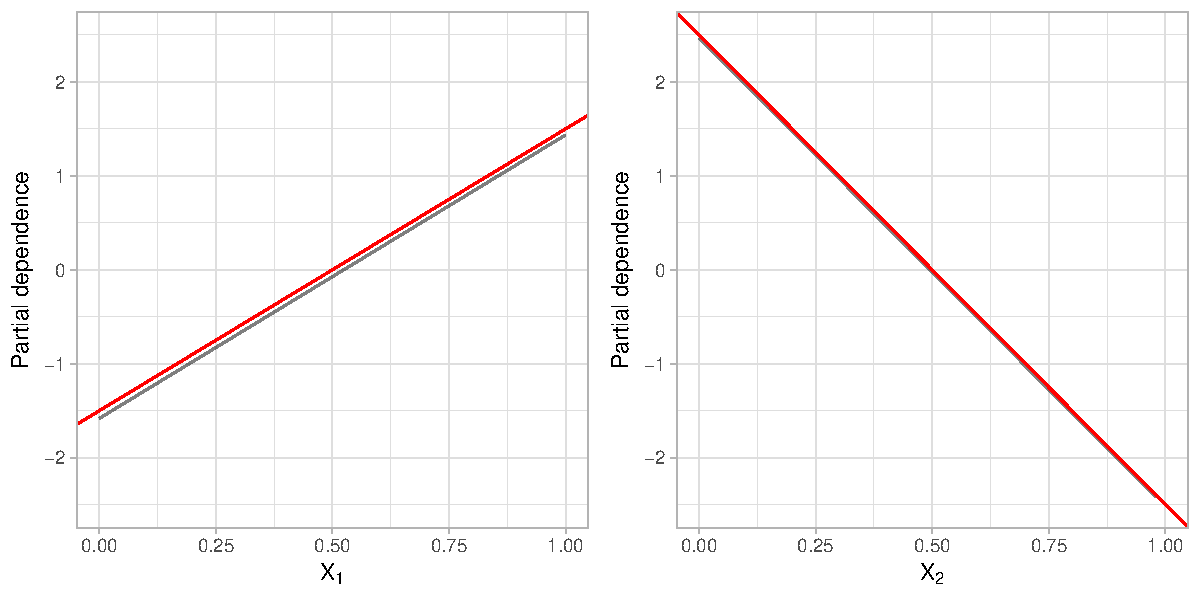
\includegraphics[width=1.0\textwidth]{lm-pdps}
  \caption{Estimated and true partial dependence plots. \label{fig:lm-pdps}}
\end{figure}

Based on these plots, $X_2$ is clearly more influential than $X_1$. Taking the absolute value of the ratio of the slopes in $f_2\left(X_2\right)$ and $f_1\left(X_1\right)$ gives $5 / 3 \approx 1.67$. In other words, $X_2$ is roughly 1.67 times more influential on $Y$ than $X_1$. Using the partial-dependence-based variable importance metric, we obtain $\imp\left(X_1\right) = 1.4828203$ and $\imp\left(X_2\right) = 0.8961719$ which gives the ratio $\imp\left(X_2\right) / \imp\left(X_1\right) \approx 1.65$. In fact, we can compute the true variance for both partial dependence functions:
\begin{equation*}
Var\left[f_1\left(X_1\right)\right] = 3^2 / 12 \quad and \quad Var\left[f_2\left(X_2\right)\right] = 5^2 / 12.
\end{equation*}
Hence, the ratio of the true standard deviations is $5 / 3 \approx 1.67$.

Using the absolute value of the $t$-statistic becomes less useful in linear models when, for example, a predictor appears in multiple terms (e.g., interaction effects and polynomial terms). The partial dependence approach, on the other hand, does not suffer from such drawbacks.


%%%%%%%%%%%%%%%%%%%%%%%%%%%%%%%%%%%%%%%%%%%%%%%%%%%%%%%%%%%%%%%%%%%%%%%%%%%%%%%%
\subsection{Detecting interaction effects}
\label{sec:interaction}
%%%%%%%%%%%%%%%%%%%%%%%%%%%%%%%%%%%%%%%%%%%%%%%%%%%%%%%%%%%%%%%%%%%%%%%%%%%%%%%%

As it turns out, our partial dependence-based variable importance measure \eqref{eqn:vi} can also be used to quantify the strength of potential interaction effects. Let $\imp\left(x_i, x_j\right)$ $\left(i \ne j\right)$ be the standard deviation of the joint partial dependence values $\bar{f}_{ij}\left(x_{ii'}, x_{jj'}\right)$ for $i' = 1, 2, \dots, k_i$ and  $j' = 1, 2, \dots, k_j$. Essentially, a weak interaction effect of $x_i$ and $x_j$ on $Y$ would suggest that $\imp\left(x_i, x_j\right)$ has little variation when either $x_i$ or $x_j$ is held constant while the other varies. 

Let $\boldsymbol{z}_s = \left(x_i, x_j\right)$, $i \neq j$, be any two predictors in the feature space $\boldsymbol{x}$. Construct the partial dependence function $\bar{f}_s\left(x_i, x_j\right)$ and compute $\imp\left(x_i\right)$ for each unique value of $x_j$, denoted $\imp\left(x_i | x_j\right)$, and take the standard deviation of the resulting importance scores. The same can be done for $x_j$ and the results are averaged together. Large values (relative to each other) would be indicative of possible interaction effects. 


%%%%%%%%%%%%%%%%%%%%%%%%%%%%%%%%%%%%%%%%%%%%%%%%%%%%%%%%%%%%%%%%%%%%%%%%%%%%%%%%
\section{Friedman's regression problem}
%%%%%%%%%%%%%%%%%%%%%%%%%%%%%%%%%%%%%%%%%%%%%%%%%%%%%%%%%%%%%%%%%%%%%%%%%%%%%%%%

To further illustrate, we will use one of the regression problems described in Friedman (1991) and Breiman (1996). The feature space consists of ten independent $\mathcal{U}\left(0, 1\right)$ random variables; however, only five out of these ten actually appear in the true model. The response is related to the features according to the formula
\begin{equation*}
Y = 10 \sin\left(\pi x_1 x_2\right) + 20 \left(x_3 - 0.5\right) ^ 2 + 10 x_4 + 5 x_5 + \epsilon,
\end{equation*}
where $\epsilon \sim \mathcal{N}\left(0, \sigma\right)$. Using the R package \pkg{nnet} \citep{venables-modern-2002}, we fit a neural network with one hidden layer containing eight units and a weight decay of 0.01 (these parameters were chosen using 5-fold cross-validation) to 500 observations simulated from the above model with $\sigma = 1$. The cross-validated $R^2$ value was 0.94.

Variable importance plots are displayed in Figure~\ref{fig:network-vip}. Notice how the Garson and Olden algorithms incorrectly label some of the features not in the true model as "important". For example, the Garson algorithm incorrectly labels $x_8$ (which is not included in the true model) as more important than $x_5$ (which is in the true model). Similarly, Oden's method incorrectly labels $x_{10}$ as being more important than $x_2$. Our method, on the other hand, clearly labels all five of the predictors in the true model as being, by far, the most important in the fitted neural network.

\begin{figure}[!htb]
  \centering
  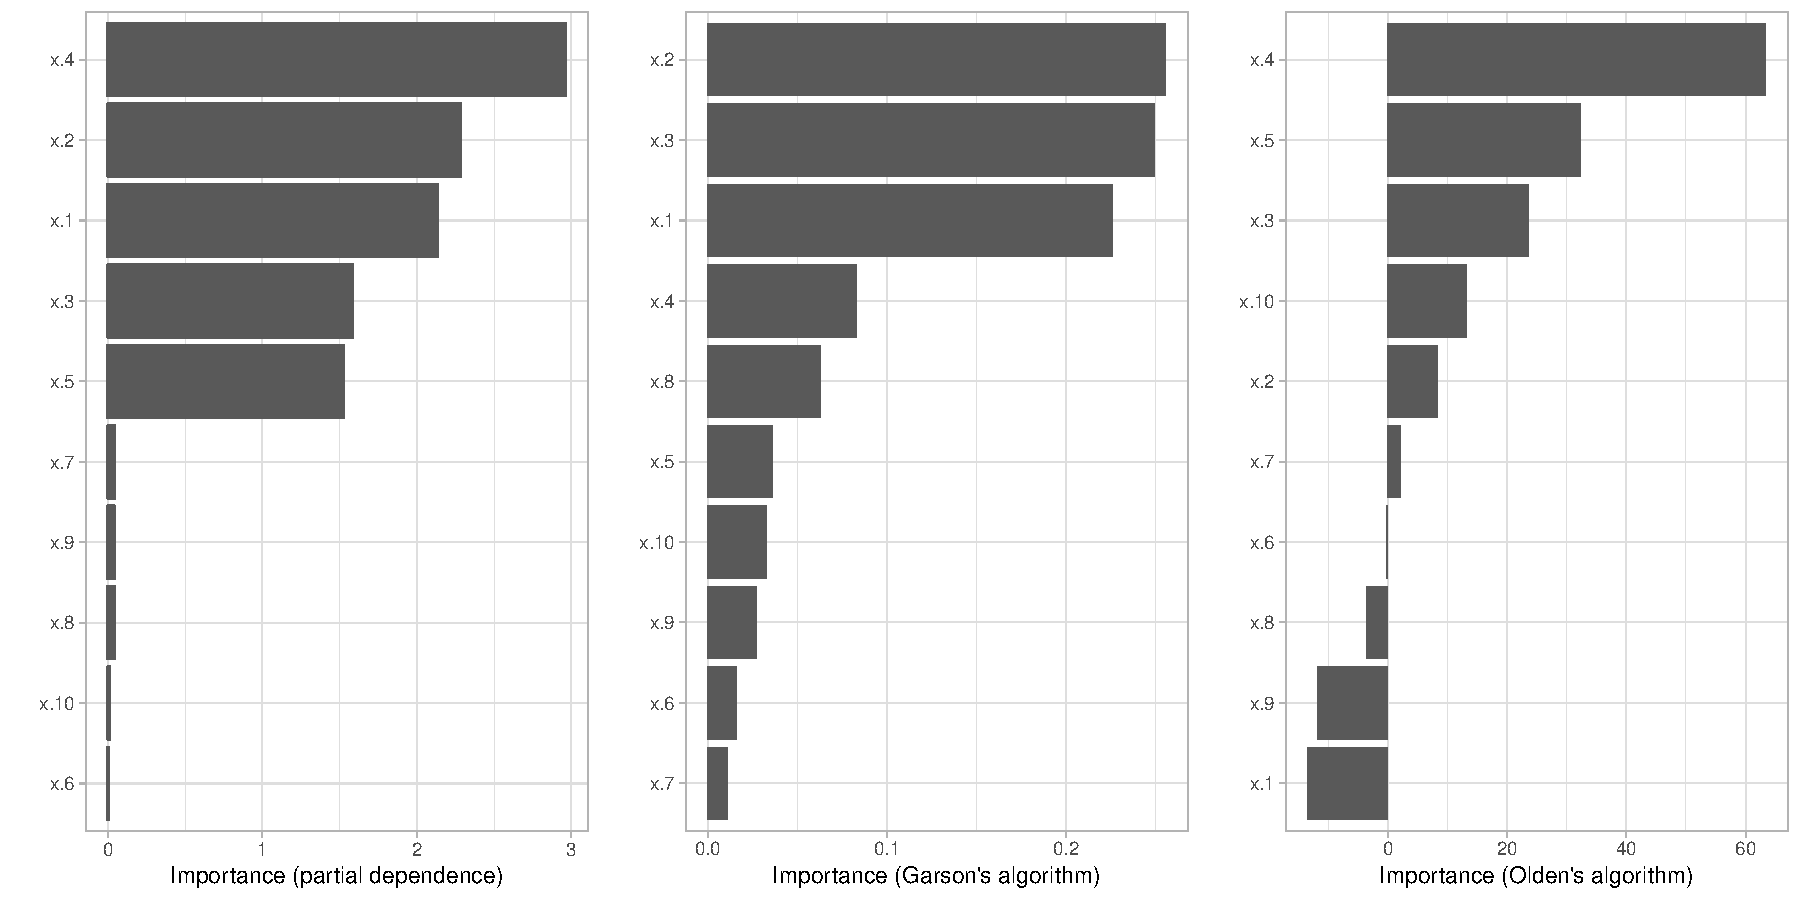
\includegraphics[width=1.0\textwidth]{network-vip}
  \caption{Variable importance plots for the neural network fit to the Friedman regression data. \textit{Left}: partial dependence-based algorithm. \textit{Middle}: Garson's algorithm. \textit{Right}: Olden's algorithm. \label{fig:network-vip}}
\end{figure}

We also constructed the partial dependence functions for all pairwise interactions and computed the interaction statistic discussed in Section~\ref{sec:interaction}. The top ten interaction statistics are displayed in Figure~\ref{fig:network-int}. There is a clear indication of an interaction effect between the predictors $x_1$ and $x_2$, the only interaction present in the true model.

\begin{figure}[!htb]
  \centering
  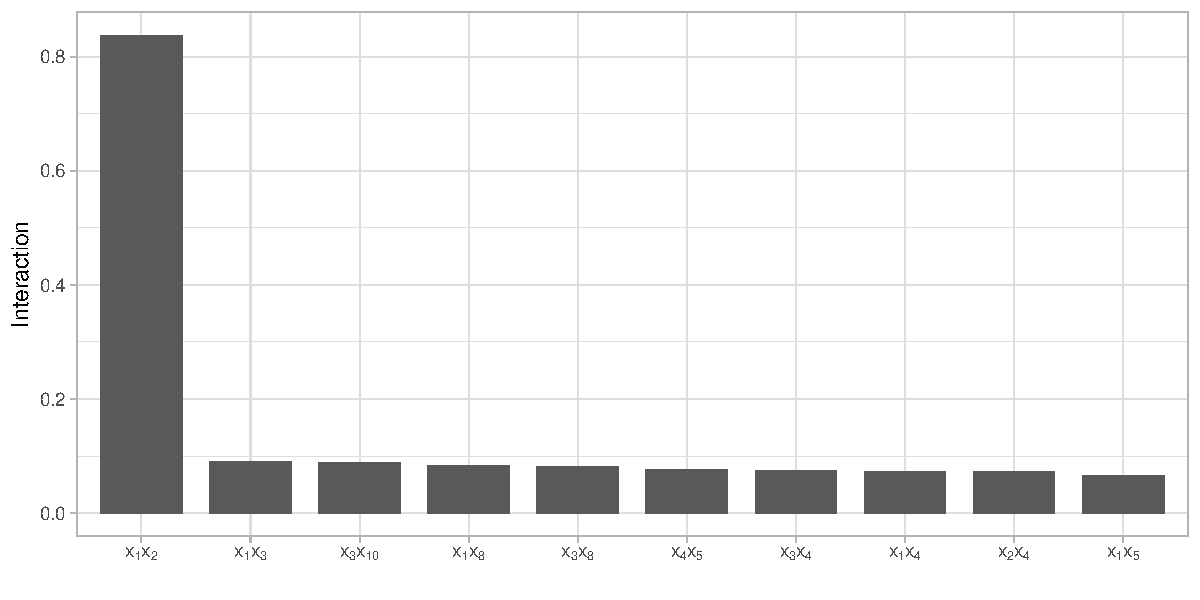
\includegraphics[width=0.75\textwidth]{network-int}
  \caption{Variable importance-based interaction statistics from the neural network fit to the Friedman regression data. \label{fig:network-int}}
\end{figure}

In fact, since we know the distributions of the predictors in the true model, we can work out the true partial dependence functions. For example, for the pairs $\left(x_1, x_2\right)$ and $\left(x_1, x_4\right)$, we have
\begin{equation*}
f\left(x_1, x_2\right) = 10 \sin \left(\pi x_1 x_2\right) + 55 / 6,
\end{equation*}
and 
\begin{equation*}
f\left(x_1, x_4\right) = \frac{5 \pi x_1 \left(12 x_4 + 5\right) - 12 \cos \left(\pi x_1\right) + 12}{6 \pi x_1}.
\end{equation*}
Next, we simulated the standard deviation of $f\left(x_1, x_2\right)$ for a wide range of fixed values of $x_2$; this is what $\imp\left(x_1 | x_2\right)$ is trying to estimate. The results from doing this for both predictors in each model are displayed in Figure~\ref{fig:interaction-simulation}. The top row of Figure~\ref{fig:interaction-simulation} illustrates that the importance of $x_1$ (i.e., the strength of its relationship to the predicted outcome) heavily depends on the value of $x_2$ and vice versa (i.e., an interaction effect between $x_1$ and $x_2$). In the bottom row, on the other hand, we see that the importance of $x_1$ does not depend on the value of $x_4$ and vice versa (i.e., no interaction effect between $x_1$ and $x_4$).

\begin{figure}[!htb]
  \centering
  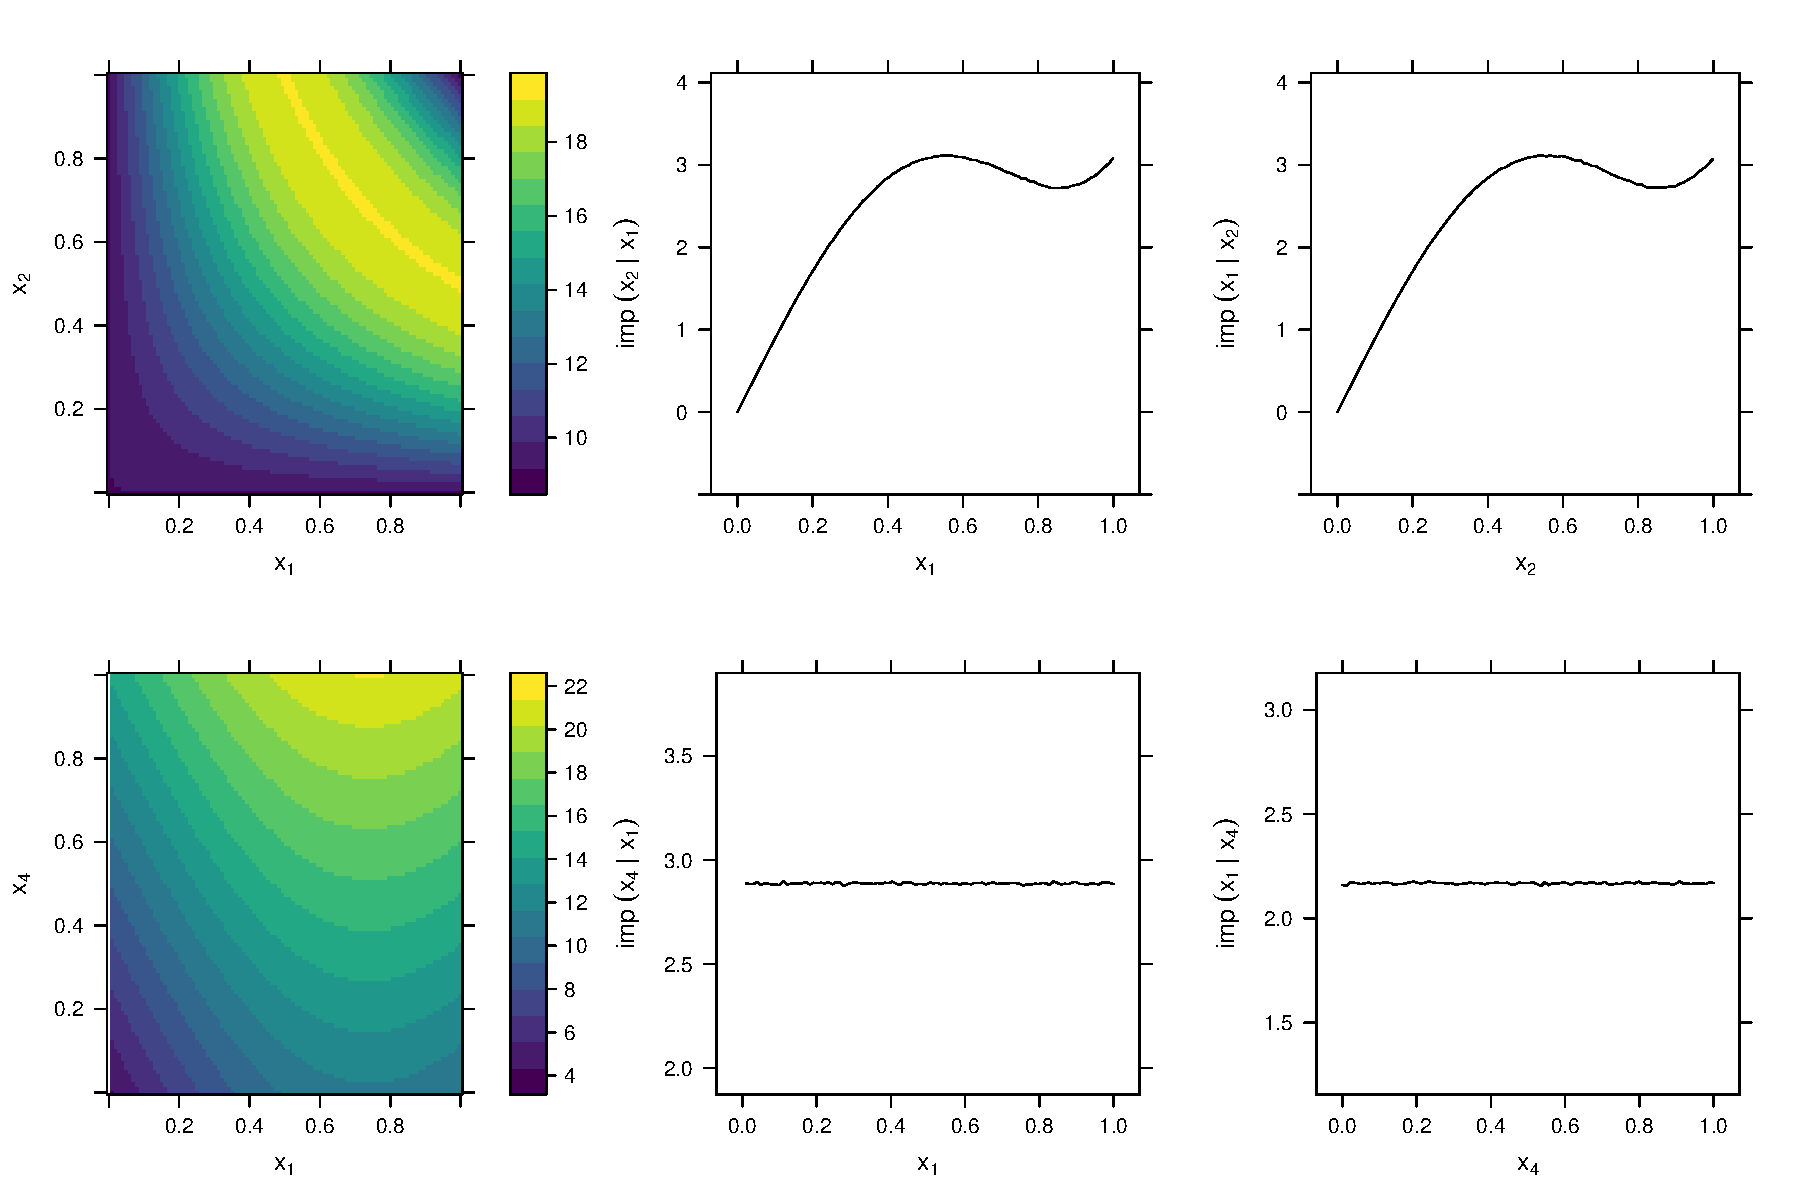
\includegraphics[width=1\textwidth]{interaction-simulation}
  \caption{Results from a small Monte Carlo simulation on the interaction effects between $x_1$ and $x_2$ (top row), and $x_1$ and $x_4$ (bottom row). \label{fig:interaction-simulation}}
\end{figure}


%%%%%%%%%%%%%%%%%%%%%%%%%%%%%%%%%%%%%%%%%%%%%%%%%%%%%%%%%%%%%%%%%%%%%%%%%%%%%%%%
\subsection{Friedman's $H$-statistic}
%%%%%%%%%%%%%%%%%%%%%%%%%%%%%%%%%%%%%%%%%%%%%%%%%%%%%%%%%%%%%%%%%%%%%%%%%%%%%%%%

An alternative measure for the strength of interaction effects is known as Friedman's $H$-statistic \citep{friedman-2008-predictive}. Coincidentally, this method is also based on the estimated partial dependence functions of the corresponding predictors, but uses a different approach.

For comparison, we fit a generalized boosted regression model (GBM) to the Friedman regression data from the previous section. The parameters were chosen using 5-fold cross-validation. We used the R package \pkg{gbm} \citep{gbm-pkg} which has built-in support for computing Friedman's $H$-statistic for any combination of predictors. The results are displayed in Figure~\ref{fig:gbm-int}. To our surprise, the $H$-statistic did not seem to catch the true interaction between $x_1$ and $x_2$. Instead, the $H$-statistic ranked the pairs $\left(x_8, x_9\right)$ and $\left(x_7, x_{10}\right)$ as having the strongest interaction effects, even though these predictors do not appear in the true model. Our variable importance-based interaction statistic, on the other hand, clearly suggests the pair $\left(x_1, x_2\right)$ as having the strongest interaction effect.

\begin{figure}[!htb]
  \centering
  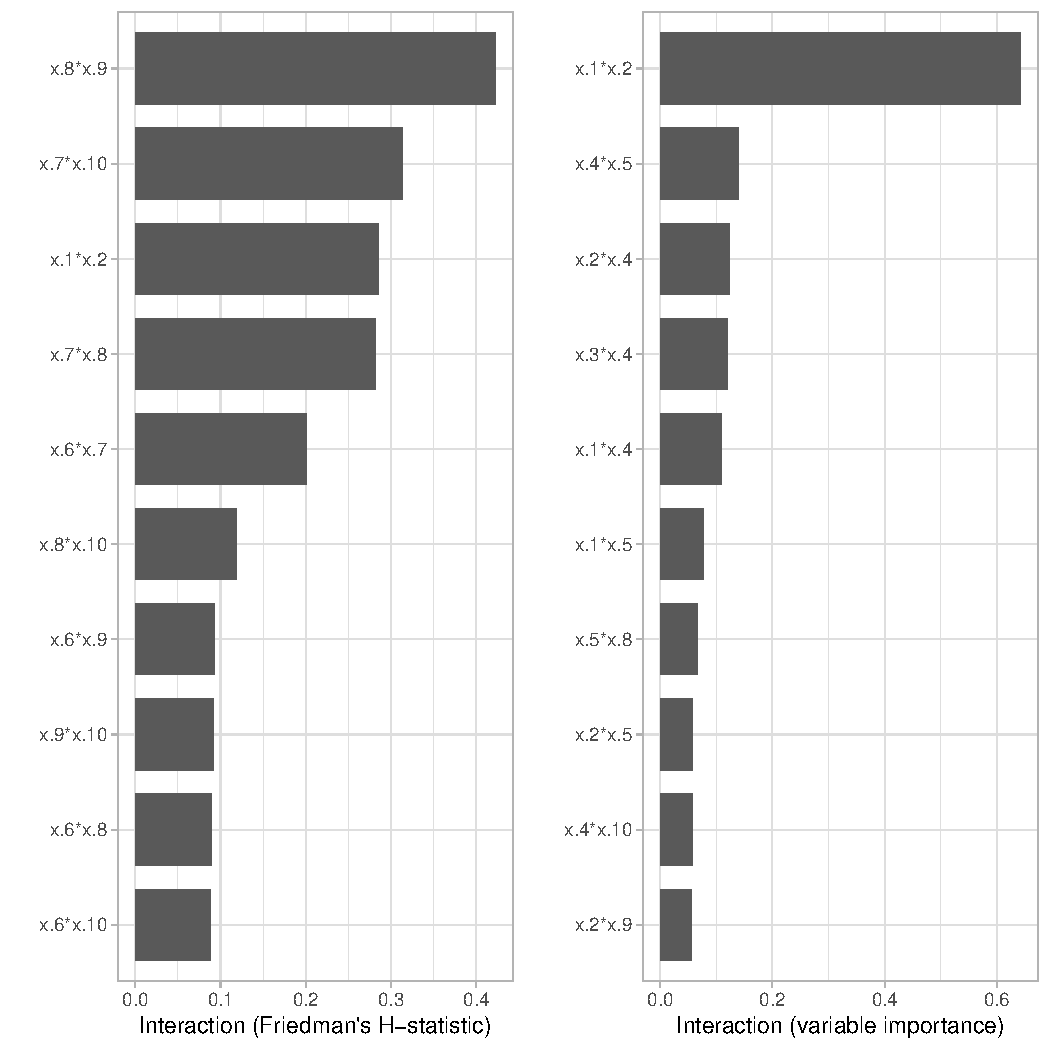
\includegraphics[width=0.75\textwidth]{gbm-int}
  \caption{Interaction statistics for the GBM model fit to the Friedman regression data. \textit{Left}: Friedman's $H$-statistic. \textit{Right}: Our variable importance-based interaction statistic. \label{fig:gbm-int}}
\end{figure}


%%%%%%%%%%%%%%%%%%%%%%%%%%%%%%%%%%%%%%%%%%%%%%%%%%%%%%%%%%%%%%%%%%%%%%%%%%%%%%%%
\section{A stacked ensemble for the Ames housing dataset}
\label{sec:ensemble}
%%%%%%%%%%%%%%%%%%%%%%%%%%%%%%%%%%%%%%%%%%%%%%%%%%%%%%%%%%%%%%%%%%%%%%%%%%%%%%%%

In the Ames housing example, we used a GBM to iilustrate the idea of using the partial dependence function to quantify the importance of each predictor on the predicted outcome (in this case, the \code{LogSalePrice}). While the GBM model acheived good a cross-validated $R^2$ of $90.06$\%, better predictive performance can often be aceived by creating an \textit{ensemble} of learning algorithms. While GBMs are themselves ensembles, we can use a method called \textit{stacking} to combine the GBM with other  cutting edge learning algorithms to form a \textit{super learner} \citep{stacked-wolpert-1992}. Such stacked ensembles tend to outperform any of the individual base learners (e.g., a single random forest or GBM) and have been shown to represent an asymptotically optimal system for learning \citep{super-laan-2003}.

For the Ames dataset, we trained and tuned a GBM and random forest using 10-fold cross-validation. The cross-validated predicted values from each of these models were combined to form a new $n \times 2$ matrix, where $n = 1460$ is the number of training records. This matrix, together with the original \code{LogSalePrice} vector, formed the ``level-one'' data. Next, we trained a \textit{metalearning} algorithm---in this case a simple generalized linear model (GLM)---on the level-one data. Two generate new predictions, first generate predictions from the random forest and GBM learners, then feed those into the GLM metalearner to generate the ensemble prediction. 

Even though the base learners in this example have the built-in capability to compute variable importance scores, there is no way of constructing them from the super learner. However, since we can generate predictions from the super learner, we can easily concstruct partial dependence functions for each predictor and use Equation~\eqref{eqn:vi}. The left and middle plots in Figure~\ref{fig:ames-ensemble-vip} display the top 15 variable importance scores from the individual base learners. The right plot displays the top 15 variable importance scores constructed using Equation~\eqref{eqn:vi} for the combined super learner. All models seem to agree on the top three predictors of \code{LogSalePrice}; namely, \code{OverallQual}, \code{Neighborhood}, and \code{GrLivArea}. 

\begin{figure}[!htb]
  \centering
  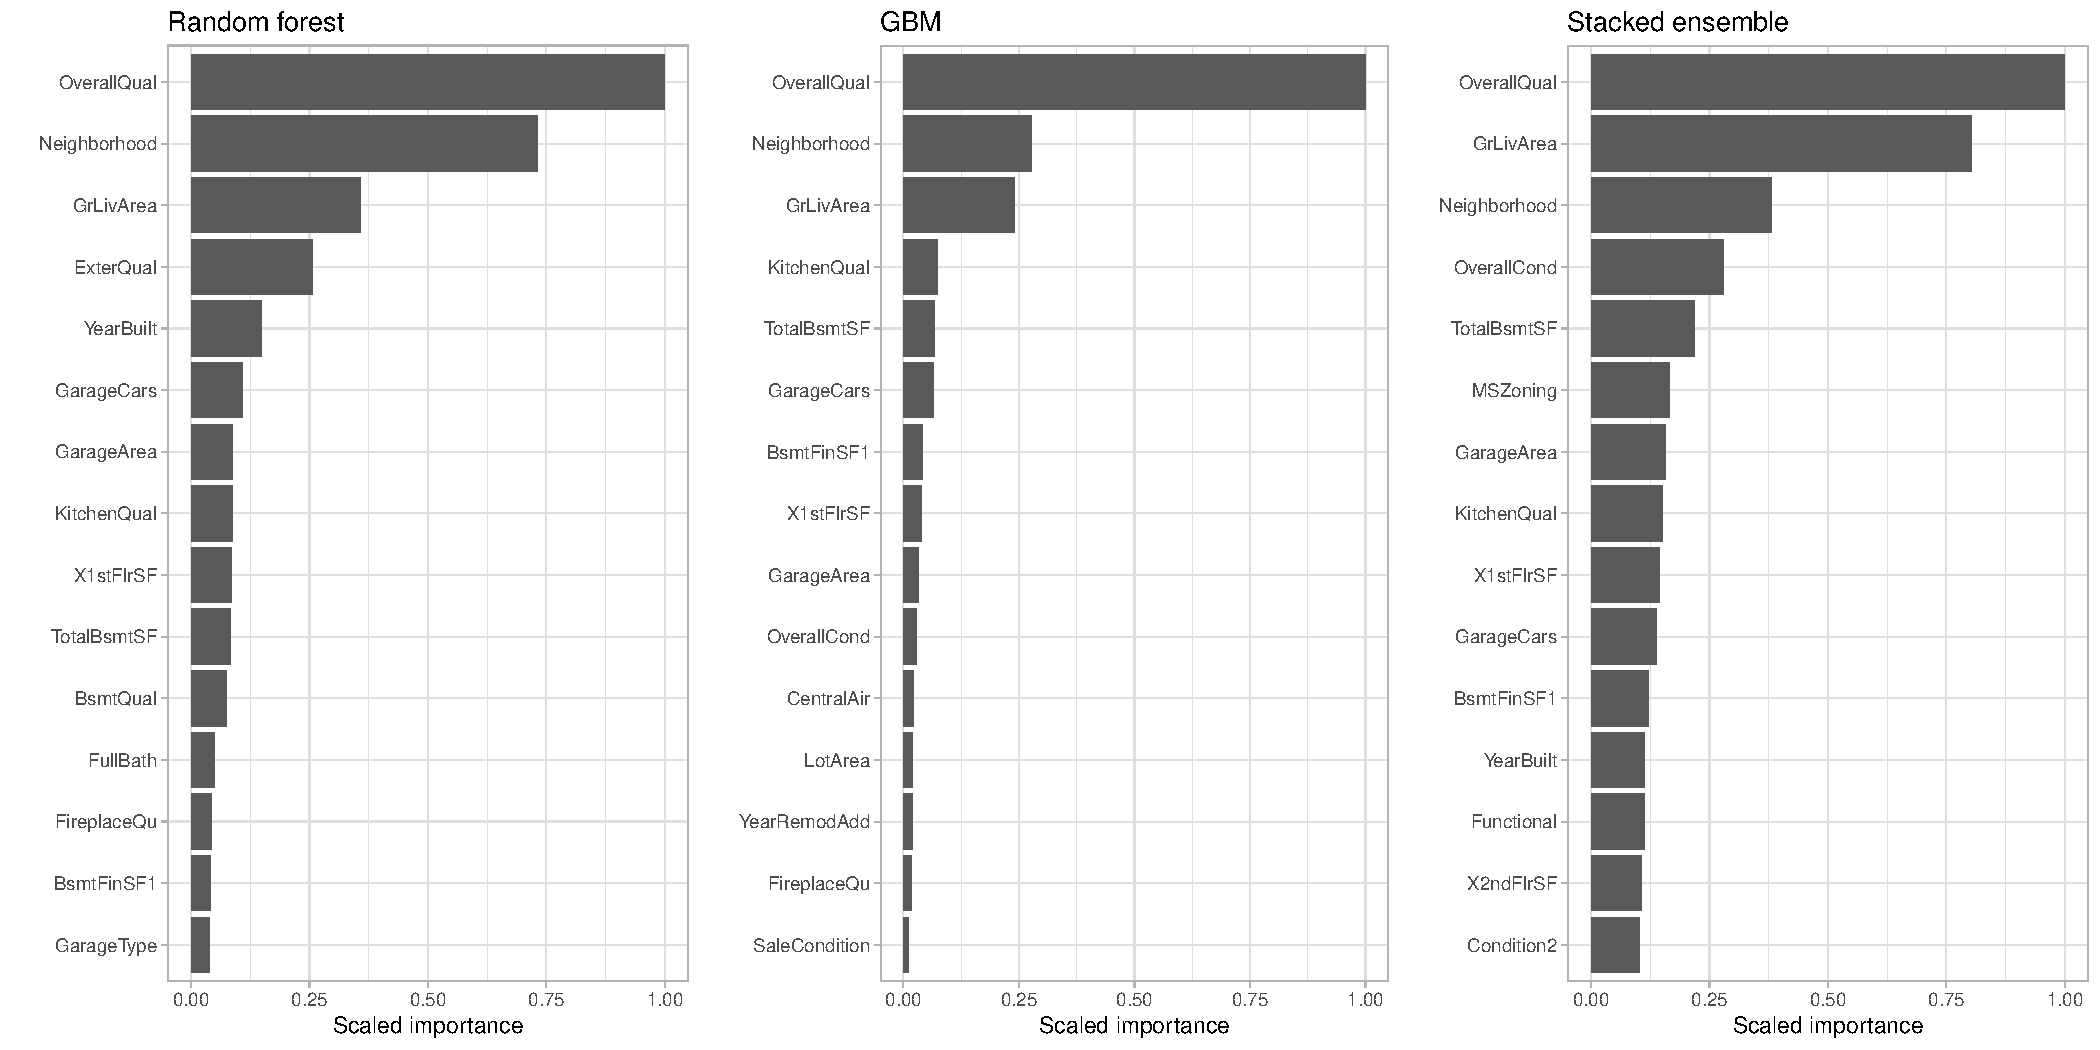
\includegraphics[width=1.0\textwidth]{ames-ensemble-vip}
  \caption{Variable importance plots for the Ames dataset. \textit{Left}: Random forest. \textit{Middle}: GBM. \textit{Right}: Stacked ensemble (i.e., super learner). \label{fig:ames-ensemble-vip}}
\end{figure}


%%%%%%%%%%%%%%%%%%%%%%%%%%%%%%%%%%%%%%%%%%%%%%%%%%%%%%%%%%%%%%%%%%%%%%%%%%%%%%%%
\section{Conclusion}
\label{sec:conc}
%%%%%%%%%%%%%%%%%%%%%%%%%%%%%%%%%%%%%%%%%%%%%%%%%%%%%%%%%%%%%%%%%%%%%%%%%%%%%%%%

We have discussed a new partial dependence-based variable important measure for supervised learning. Since our algorithm is based on Friedman's idea of partial dependence functions, it is model-based and takes into account the effects of the other features in the model. Consequently, this also requires that the fitted models be properly tuned to achieve optimum performance. We have also discussed a simple extension of our variable importance metric that seems useful for detecting interaction effects.

While this new approach to appears to have high utility, more research is needed to determine where its deficiencies may lie. For example, outliers in the feature space can cause abnormally large fluctuations in the partial dependence values $\bar{f}\left(x_{i}\right)$ $\left(i = 1, 2, \dots, k\right)$. Therefore, it may be advantageous to use more robust measures of spread to describe the variability in the estimated partial dependence values; a reasonable choice would be the median absolute deviation which has a finite sample breakdown point of $\left\lfloor{n / 2}\right\rfloor / n$. As mentioned in \citet{pdp-greenwell-2017}, it is also possible to replace the mean in step (3) of Algorithm~\ref{alg:pdp} with a more robust estimate such as the median or trimmed mean. It would also be interesting to see if our metric could be extended to rely on individual conditional expectation (ICE) curves \citep{goldstein-peeking-2015}, a refinement over Friedman's PDP.


%%%%%%%%%%%%%%%%%%%%%%%%%%%%%%%%%%%%%%%%%%%%%%%%%%%%%%%%%%%%%%%%%%%%%%%%%%%%%%%%
% Supplementary material
%%%%%%%%%%%%%%%%%%%%%%%%%%%%%%%%%%%%%%%%%%%%%%%%%%%%%%%%%%%%%%%%%%%%%%%%%%%%%%%%

\bigskip
\begin{center}
{\large\bf SUPPLEMENTARY MATERIAL}
\end{center}

\begin{description}

\item[R package:] The R package \pkg{vip}, hosted on GitHub at \url{https://github.com/AFIT-R/vip}, contains functions for computing variable importance scores and constructing variable importance plots for various types of fitted models in R using the method discussed in this paper.

\item[R code:] The R script \file{greenwell-vi-2017.R} contains the R code to reproduce all of the results and figures in this paper.

\end{description}


%%%%%%%%%%%%%%%%%%%%%%%%%%%%%%%%%%%%%%%%%%%%%%%%%%%%%%%%%%%%%%%%%%%%%%%%%%%%%%%%
% Bibliography
%%%%%%%%%%%%%%%%%%%%%%%%%%%%%%%%%%%%%%%%%%%%%%%%%%%%%%%%%%%%%%%%%%%%%%%%%%%%%%%%

\bibliographystyle{Chicago}

\bibliography{greenwell-vi-2017}
\end{document}
